\documentclass[../../../main.tex]{subfiles}
\graphicspath{{sections/part2/images/}}
\begin{document}
\definition{Flot d'exécution/de contrôle}{Le flot d'exécution ou flot de contrôle est l'ordre dans lequel les instructions d'un programme impératif sont exécutés. Il est possible de modifier cet ordre grâce à des structures de contrôle de flot.}

Un programme informatique est constitué d'une succession d'instruction binaires chacune chargée en mémoire. Il existe dans le processeur un registre qui stocke l'adresse de l'instruction à exécuter.\newline
Ce registre est appelé par différents noms :
\begin{itemize}
	\item \textit{PC} pour \textit{\underline{P}rogram \underline{C}ounter}
	\item \textit{IP} pour \textit{\underline{I}nstruction \underline{P}ointer}
	\item \textit{IAR} pour \textit{\underline{I}nstruction \underline{A}ddress \underline{R}egister}
\end{itemize}
La manipulation de la valeur ce registre permet de se ``déplacer'' dans le programme. Ces modes de déplacements sont décrits dans les sections suivantes.
 
\begin{minipage}{\textwidth}
	\begin{center}
		\includesvg[width=0.75\textwidth]{instruction_pointer}
	\end{center}
\end{minipage}
 
La première sous-section se veut une introduction plus bas-niveau du contrôle du flot d'exécution, c'est-à-dire détaillant de manière moins abstraite et plus technique le contrôle du flot d'exécution.\footnote{Il s'agit d'une introduction légère au cours d'architecture des processeurs} Il est possible d'aller directement à la sous-section décrivant les structures complexes, majoritairement utilisées en langage C.
\subsection{Structures élémentaires}
Voir \cite{CSaPP} pour plus de détails.

Un ordinateur utilise les structures élémentaires de contrôle de flot suivantes :
\begin{itemize}
	\item la séquence
	\item l'arrêt de programme
	\item le saut inconditionnel
	\item le saut conditionnel
\end{itemize}
Les structures de contrôle plus abstraites sont ensuite construites par l'utilisation de ces structures élémentaires.

\subsubsection{Séquence}
 
La séquence est une structure de contrôle implicite, dont la gestion est réservée au processeur de l'ordinateur. Il s'agit simplement du passage d'une instruction à la suivante. En langage C, c'est le point-virgule indiquant la fin d'une instruction qui se charge d'indiquer le passage à la suivante.
 
La fin d'un instruction va donc amener à l'incrémentation du registre \textit{IP} de la taille de l'instruction. Imaginons que le processeur exécute la $i^e$ instruction de taille $t_{i}$ octets à l'adresse $a_{i}$. À l'exécution de cette instruction, $IP = a_{i}$. À la fin de l'exécution de l'instruction, $\textit{IP} = a_{i} + t_{i} = a_{i+1}$. Il s'agit de l'adresse de l'instruction suivante, puisque toutes les instructions sont contigües en mémoire.
 
Certaines architectures de processeur utilisent une taille fixe pour les instructions. Dans ce cas, $\forall{i}, t_{i} = k\in{\mathbb{N}}$ est une constante. Cela accélére l'accès aux instructions par le processeur, mais limite le nombre possible d'instructions.\footnote{Par exemple, les processeurs Intels utilisent des instructions de taille variable tandis que les processeurs ARM utilisent des instructions de taille fixe}
 
\subsubsection{Arrêt de programme}
 
La mise en pause d'un programme à un certain point de son exécution et sa reprise est nécessaire pour un système multi-tâches qui doit exécuter plus de programmes au même moment qu'il ne possède de processeurs. Il peut ainsi alterner l'exécutions des programmes pour simuler leur exécution parallèle aux yeux de l'utilisateur. On peut imaginer \textit{par exemple} deux programmes utilisant chacun pendant $10\ ms$ les ressources de l'ordinateur. Ils ne s'exécuteront que $500\ ms$ chacun pendant une seconde, mais l'utilisateur pensera du fait de l'alternance très rapide d'exécution des programmes que ceux-ci s'exécutent en même temps (deux fois plus lentement cependant que si ils avaient été seuls à utiliser les ressources du processeur).
 
\subsubsection{Saut inconditionnel}
 
Le saut inconditionnel consiste à attribuer au registre \textit{IP} une valeur précisée dès que l'instruction est lue, sans aucune condition. Le processeur passe donc immédiatement à l'instruction souhaitée.
 
En langage C, l'instruction qui permet d'effectuer ce genre de saut est \textsf{goto}. Il faut lui préciser une adresse d'instruction du code C qui sera indiqué par un \textit{label} définie selon la syntaxe suivante :
\begin{minted}[linenos=false]{c}
mon_label:
\end{minted}
Un exemple :
\begin{minted}{c}
#include <truc.h>

int main() {
	goto fin;
	// ici : opérations jamais exécutées
fin:
	operations_de_fin();
	return EXIT_SUCCESS;
}
\end{minted}
Pensez à oublier ça, c'était pour la culture, mais sauf à faire de l'assembleur, il faut éviter\dots
 
\subsubsection{Saut conditionnel}
 
Le processeur contient un registre appelé le registre des \textit{drapeaux} (\textit{flags} en anglais), ou registre de statut. Ces \textit{drapeaux}, ou statuts, permettent d'indiquer des états du processeur vis-à-vis des actions qu'il a effectué. Chaque statut est stocké dans un bit du registre. On note $N$ le nombre de bits du registre ($N$ peut varier selon le processeur).
$$R_{flags} = s_{N-1}\dots s_{0}$$
Chaque instruction du processeur va modifier certains bits du registre. Par exemple, lors de l'addition de deux nombres non signés $a$ et $b$ stockés dans des registres 32 bits, si $a + b > 2^{32} - 1$, le drapeau dit de retenue (\textit{carry flag} en anglais, noté CF dans la littérature) sera mis à 1.
 
\urldef{\urlrflagsa}\url{https://wiki.osdev.org/CPU_Registers_x86#EFLAGS_Register}
\urldef{\urlrflagsb}\url{https://en.wikipedia.org/wiki/FLAGS_register}
Le saut conditionnel consiste à attribuer au registre \textit{IP} une valeur précisée lorsque l'instruction est lue, à la condition qu'un certain drapeau du registre des drapeaux ait une certaine valeur (0 ou 1).\footnote{voir \urlrflagsa et \urlrflagsb pour une liste des drapeaux des processeurs Intels} On peut ainsi vérifier :
\begin{itemize}
	\item l'égalité entre deux nombres $a$ et $b$ (en vérifiant $a - b = 0$ ou $a - b \neq{0}$)
	\item l'inégalité entre deux nombres $a$ et $b$ (en vérifiant $a - b > 0$ ou $a - b < 0$)
	\item \textit{et caetera}\dots
\end{itemize}
Il est ainsi possible de former des conditions pour contrôler le flot d'exécution. L'exemple suivant est écrit en NASM pour un processeur Intel 64 bits. Il s'agit d'un langage assembleur, dont chaque instruction correspond donc de manière directe à une instruction exécutée par le processeur :
\begin{minted}{nasm}
; point-virgules pour les commentaires

section .text ; début du programme
	global _start

_start: ; pareil que fonction 'main' en C

mov al, 200 ; al est un registre 8 bits, et 2^8 = 256
add al, 100 ; 200 + 100 > 256, donc CF = 1
jc fin ; JC signifie Jump if Carry -> saute si retenue
	; le code ici est ignoré car CF != 0
fin: ; le code qui suit clôt l'exécution du programme
mov rax, 231
mov rdi, 0
syscall
\end{minted}
\textsf{end} est une étiquette choisie par le programmeur. Elle permet de nommer l'adresse mémoire d'une instruction. Elle est traduite à la ``compilation'' du code ci-dessus en adresse mémoire. Le code en NASM est équivalent au pseudo-code suivant :
\begin{algorithm}
\caption{Traduction en pseudo-code}\label{alg:two}
$al\leftarrow 200$\;
$al\leftarrow al + 100$\;
\eSi{la dernière opération a effectué un dépassement de capacité} {
	Aller à la fin du programme\;
} {
	Les instructions ici sont sautés
}
Fin du programme\;
\end{algorithm}\newline
On pourrait alors imaginer la boucle suivante : (voir \textit{boucle for} dans les structures abstraites)
\begin{minted}{nasm}
; ...
mov al, 10
boucle:
; trucs à répéter 10 fois
sub al, 1
jnc boucle ; saute si al - 1 >= 0
fin_de_boucle:
; ...
\end{minted}
\subsection{Structures complexes}
Grâce aux structures élémentaires de contrôle de flot d'exécution, le langage C propose des structures de contrôle beaucoup plus intuitives dans leur utilisation :
\begin{itemize}
	\item les conditions
	\begin{itemize}
	\item le branchement \textsf{if-else}
	\item l'aiguillage
	\end{itemize}
	\item les boucles
	\begin{itemize}
		\item la boucle à pré-condition
		\item la boucle à post-condition
		\item la boucle itérative
	\end{itemize}
\end{itemize}
Les détails de la construction de ces structures abstraites ne seront pas décrits ici. Cela peut en effet dépendre du compilateur.\footnote{Un exemple d'une possibilité d'implantation est cependant donné au dessus en langage assembleur}

Les \textit{conditions} permettent au programme d'effectuer des choix quant à son flot d'exécution et ainsi de ne pas être entièrement séquentiel.

Les \textit{boucles} permettent d'effectuer un bloc d'instructions plusieurs fois de suite. Par exemple, trouver le minimum d'un ensemble de nombres nécessite de parcourir tous ces nombres, et il serait un peu ennuyant d'avoir à d'écrire autant d'instructions qu'il y a d'éléments de cet ensemble, surtout si celui-ci contient des milliers voire des millions de nombres.
\subsubsection{Branchement \textsf{if-else} :}
 
Le branchement \textsf{if-else} consiste à n'exécuter une partie du code que si une certaine condition est satisfaite, et en exécuter une autre si cette condition n'est pas satisfaite. On observe ainsi le pseudo-code suivant :
\begin{algorithm}
\caption{Branchement conditionnel}
\eSi{$condition \neq{0}$} {
	Instructions si $condition \neq{0}$
} {
	Instructions si $condition = 0$
}
Suite du programme
\end{algorithm}
En langage C, cela donne :
\begin{minted}[linenos=false]{c}
if (condition) {
	printf("La condition est verifiee.\n");
} else {
	printf("La condition n'est pas verifiee.\n");
}
printf("Suite du programme\n");
\end{minted}
On remarque que $\neq{0}$ est implicite. Ainsi, les deux codes suivants sont équivalents :

\begin{minipage}{0.5\textwidth}
\begin{minted}[linenos=false]{c}
int a = 4;
int b = 6;
if (a - b) {
	printf("a different de b.");
} else {
	printf("a = b");
}
\end{minted}
\end{minipage}
\begin{minipage}{0.5\textwidth}
\begin{minted}[linenos=false]{c}
int a = 4;
int b = 6;
if (a - b != 0) {
	printf("a different de b.");
} else {
	printf("a = b");
}
\end{minted}
\end{minipage}
 
On pourrait aussi écrire de manière plus lisible : 
 
\begin{minipage}{0.5\textwidth}
\begin{minted}[linenos=false]{c}
int a = 4;
int b = 6;
if (a != b) {
	printf("a different de b.");
} else {
	printf("a = b");
}
\end{minted}
\end{minipage}
\begin{minipage}{0.5\textwidth}
\begin{minted}[linenos=false]{c}
int a = 4;
int b = 6;
if ((a != b) != 0) { // ou a != b != 0
	printf("a different de b.");
} else {
	printf("a = b");
}
\end{minted}
\end{minipage}
 
Par ailleurs, l'instruction \textit{else} est tout à fait optionnelle. L'omettre signifie simplement qu'il n'y a rien à exécuter si la condition n'est pas vérifiée :
\begin{minted}[linenos=false]{c}
int a = 4;
int b = 6;
if (a > b) { // ou a != b != 0
	printf("?");
}
printf("texte par defaut"); // sera toujours exécuté
\end{minted}
Il est également possible d'enchaîner plusieurs blocs de branchements conditionnels :
\begin{minted}[linenos=false]{c}
int a = 4;
int b = 6;
if (a > b) { // ou a != b != 0
	printf("%d > %d\n", a, b);
} else if (a == b) {
	printf("egaux\n");
} else {
	printf("%d > %d\n", b, a);
}
printf("texte par defaut"); // sera toujours exécuté
\end{minted}
\subsubsection{Opérateur ternaire}
 
L'opérateur ternaire permet d'écrire certaines conditions de manière compacte :
 
\begin{minipage}{0.65\textwidth}
\begin{minted}[linenos=false]{c}


variable = (condition) ? expression_1 : expression_2;


\end{minted}
\end{minipage}
\begin{minipage}{0.35\textwidth}
\begin{minted}[linenos=false]{c}
if (condition) {
	variable = expression_1;
} else {
	variable = expression_2;
}
\end{minted}
\end{minipage}
 
Il y a stricte équivalence sémantique entre la syntaxe à gauche et celle à droite. Cela questionne évidemment les raisons de l'existence d'une telle syntaxe en C, mise à part la compacité de l'écriture.
 
La raison, assez technique\footnote{Pour les curieux, voir \url{https://drive.google.com/file/d/1bkLb3OByL_UaBNz-ksr03WliZ6mnuiy-/view?usp=drive_link}}, sera simplement réduite à ses conséquences : l'utilisation d'une condition ternaire permet d'optimiser la vitesse d'exécution des instructions par l'UCC\footnote{Il faut préciser que le compilateur effectue le plus souvent lui-même l'optimisation si vous oubliez d'utiliser une condition ternaire.}.
 
Un petit exemple d'utilisation :
\begin{minted}{c}
// <math.h> nécessite l'option -lm
// à la fin de la ligne de commande pour compiler :
// gcc main.c -o main -lm
#include <stdlib.h>
#include <math.h> // NaN (Not A Number), sqrt

int main() {
	double a = ...; // valeurs
	double b = ...; // quelconques
	double c = ...;

	// Résoud une équation à solutions réelles de degré 2
	double d = b*b - 4*a*c;
	double x1 = (d < 0) ? NAN : (-b - sqrt(d))/(2*a);
	double x2 = (d < 0) ? NAN : (-b + sqrt(d))/(2*a);

	return EXIT_SUCCESS;
}
\end{minted}
\subsubsection{Aiguillage}
 
L'aiguillage est une autre forme de branchement conditionnel. Il permet de diriger le flot d'exécution selon la valeur d'une variable entière. On peut vouloir associer à plusieurs nombres un bloc d'instructions différent. L'aiguillage permet de faire correspondre à des entiers des blocs d'instructions.
 
Il posséde quelques avantages et inconvénients :
\begin{itemize}
	\item avantages :
	\begin{itemize}
		\item très lisible
		\item permet une optimisation plus poussé du code par le compilateur
		\item facilite l'écriture des conditions sur des structures complexes (parce-que personne n'a envie d'écrire 40 \textsf{if-else} enchaînés les uns dans les autres)
	\end{itemize}
	\item inconvénients : 
	\begin{itemize}
		\item ne test que des égalités
		\item les valeurs à égaler doivent être écrites en dur
	\end{itemize}
\end{itemize}
Cet aiguillage sert en général à effectuer un choix, qu'il s'agisse du parcours d'une structure informatique complexe\footnote{Patience et longueur de temps font plus que force ni que rage, a écrit un type un jour\dots Faut attendre un peu avant de faire des trucs impressionants, z'inquiétez pas ça va arriver}, ou d'un simple menu dans l'application d'un restaurant.
 
En langage C, l'aiguillage est introduit par le mot-clé \textsf{switch}. Les mot-clés \textsf{case} et \textsf{break} viennent avec.
\begin{minted}[linenos=false]{c}
unsigned int x;
switch (x) {
case 0:
	printf("Choix 0");
	// et d'autres instructions
	break;
case 1:
case 2:
	printf("Choix 1 ou 2");
	// et d'autres instructions
	break;
case 3:
	printf("Choix 3 puis 4");
	// et d'autres instructions
case 4:
	printf("Choix 4");
	// et d'autres instructions
	break;
default:
	printf("Autre");
	// et d'autres instructions
	break;
}
printf("apres le switch");
\end{minted}
L'exemple ci-dessus se veut exhaustif des cas possibles de l'instruction \textsf{switch}. On observe que le flot d'exécution va ``sauter'' au \textsf{case} correspondant à la valeur de $x$, et à \textsf{default} si cette valeur n'est pas présente dans l'aiguillage. \textit{L'exécution redevient séquentielle à partir de cet instant !} Une erreur régulièrement faite par les débutants est de penser qu'à la fin de l'exécution du \textsf{case}, le flot vient tout de suite après le switch. Cela n'est pas vrai sans le mot-clé \textsf{break} qui ``casse'' le bloc d'instructions en cours d'exécution et saute à la fin.
 
Dans l'exemple ci-dessus, l'exécution du code pour $x = 3$ est suivie immédiatement par l'exécution du code pour $x = 4$ car il n'y a pas de \textsf{break}. De la même manière, si $x = 1$, le flot va sauter à la ligne \textsf{case 1} puis va séquentiellement avancer au bloc d'instructions pour $x = 2$.
\subsubsection{Boucle à pré-condition (ou boucle \textit{while}) :}
La boucle à pré-condition suit le pseudo-code suivant :
\begin{algorithm}
\caption{Boucle \textit{While}}
\Tq {$condition \neq{0}$} {
	Instructions
}
\end{algorithm}
\newline
Il s'agit d'une boucle qui vérifie \textit{avant} l'exécution du bloc d'instructions qu'une certaine condition est vérifiée, et exécute ainsi le bloc d'instruction jusqu'à ce que la condition ne soit plus vérifiée. C'est le contenu de ce bloc d'instructions qui va amener à ce que la condition ne soit plus satisfaite.
\begin{minted}[linenos=false]{c}
while (condition) {
	// bloc d'instructions exécutés tant que (condition != 0)
}
\end{minted}
Comme pour le branchement \textsf{if-else}, la différence à 0 de la condition est implicite.
 
On peut par exemple imaginer le code suivant :
\begin{minted}{c}
#include <stdio.h>
#include <stdlib.h>

#define N ...

int main() {
	int u = 3;
	unsigned int n = 0;
	while (n < N) {
		u = 3*u*u - 5*u + 2;
		n++; // n++ <=> n += 1
	}
	printf("u(%u) = %d\n", n, u);
	return EXIT_SUCCESS;
}
\end{minted}
Ce programme calcule l'élément de rang $N$ précisé de la suite $(u_{n})_{n\in{\mathbb{N}}}$ définie telle que :
$$
\left\{\begin{array}{llcl}
& u_{0} & = & 3 \\
\forall{n\in{\mathbb{N}}}, & u_{n+1} & = & 3u_{n}^{2} - 5u_{n} + 2
\end{array}\right.
$$
\exercise{[COURS]} Modifier le programme donné en exemple pour qu'il affiche toutes les valeurs $u_{1}, \dots, u_{N}$. \newline
Expliquer pourquoi les valeurs deviennent fausses à partir d'un certain rang que l'on précisera.
 
\subsubsection{Boucle à post-condition (ou boucle \textit{do-while})}
 
La boucle à post-condition est pratiquement identique à la boucle à pré-condition, à une nuance qui a son importance : la condition est effectuée à la fin de l'exécution de la boucle. Cela signifie qu'au contraire de la boucle à pré-condition, le bloc d'instructions d'une boucle à post-condition s'exécute au moins une fois. Les deux codes suivants sont donc équivalents :
 
\begin{minipage}{0.5\textwidth}
\begin{minted}[linenos=false]{c}
do {
	// Bloc d'instructions
} while (condition);

\end{minted}
\end{minipage}
\begin{minipage}{0.5\textwidth}
\begin{minted}[linenos=false]{c}
// Bloc d'instructions
while (condition) {
	// Même bloc d'instructions
}
\end{minted}
\end{minipage}
 
Ce type de boucle est extrêmement utile quand on veut être certain qu'une action est effectuée au minimum une fois. Par exemple, il peut s'agir de demander à un utilisateur d'entrer des nombres jusqu'à ce que l'utilisateur entre le nombre $0$.
 
\subsubsection{Boucle itérative (ou boucle \textit{for})}
 
La boucle itérative est un cas particulier de boucle à pré-condition. Elle est construite selon le format suivant en langage C :
\begin{minted}[linenos=false]{c}
for (initial; condition; pas) {
	// Bloc d'instructions
}
\end{minted}
et est équivalente au pseudo-code suivant :
\begin{algorithm}
\caption{Boucle \textit{for}}
Exécuter l'instruction initiale\;
\Tq {condition} {
	Instructions \Comment*[r]{Bloc d'instructions}
	Instruction de pas \Comment*[r]{Puis le pas}
}
\end{algorithm} \newline
L'idée est en générale d'utiliser l'instruction de \textit{pas} pour parcourir une structure. Il s'agit d'une itération sur un élément de parcours, raison qui donne son nom à cette syntaxe de boucle. Son application va être vue dans la section sur les \textit{tableaux}.
 
\textbf{Remarque 1 :} \textsf{initial} et \textsf{pas} ne peuvent être au maximum constitués que d'une instruction.
 
\textbf{Remarque 2 :} \textsf{initial}, \textsf{condition} et \textsf{pas} sont optionnels, tout comme le bloc d'instruction. Si la condition est oubliée, elle est considérée comme toujours vraie.
 
Quelques exemples :
\begin{minted}[linenos=false]{c}
// Boucle infinie :
for (;;) {
	
}

// Boucle infinie incrémentant une variable :
for (int a = 0; ; a++) { // a++ <=> a += 1
	
}

// Boucle finie qui démarre en affichant du texte
int a;
for (printf("Initialement, a = %d\n", a = 1); a < 10; printf("À présent : a = %d\n", ++a));
\end{minted}

\subsection{Détails sur l'instruction \textbf{break} (et l'instruction \textbf{continue})}
L'instruction \textsf{break} a été rapidement vue pour l'aiguillage. Mais une question -- légitime -- subsiste quand aux blocs d'instructions qui peuvent être "cassés" et ceux qui ne peuvent l'être.

La réponse tient simplement : l'instruction \textsf{break} casse les blocs d'instructions \textsf{while}, \textsf{do-while}, \textsf{for} et \textsf{switch}, sans aucune exception. Le contrôle du programme est ensuite directement rendu à la première instruction suivant le bloc. Par exemple :
\begin{minted}[linenos=false]{c}
#define N 28

...

unsigned int i = 0;
while (1) {
	if (i*i >= N) {
		break;
	}
	i++;
}
printf("Plus petit i tel que i*i >= %u : %u", N, i); // -> 6
\end{minted}

L'instruction \textsf{continue} est le dual de l'instruction \textsf{break} pour les blocs \textsf{while}, \textsf{do-while} et \textsf{for} -- mais pas pour les \textsf{switch}. L'instruction \textsf{continue} permet de sauter à la première instruction de la boucle, \textit{sans exécuter le test de boucle}\footnote{Ce qui rend compatible l'instruction avec les boucles \textsf{do-while}}.

\textbf{\color{red}Mais pourquoi on utilise jamais \textsf{goto} ? C'est plus basique donc c'est mieux ?}

\begin{minipage}{\textwidth}
	\begin{center}
		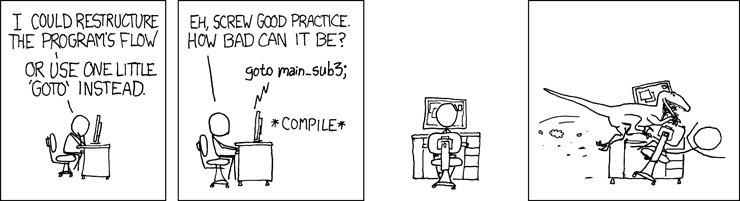
\includegraphics[width=\textwidth]{meme2}
	\end{center}
\end{minipage}
 
Plus sérieusement, il est vraiment recommandé de ne jamais faire cela. En effet, ce genre de saut est effectué sans contrôle (donc augmente les risques de bogues) et permet moins d'optimisations de la part du compilateur car son fonctionnement ne possède pas de logique intrinsèque, au contraire des boucles \textit{for} et \textit{while} qui suivent des règles contraintes par des conditions.

\subsection{Exercices}
Dans la suite, $N$ désigne une constante définie par un \textsf{\#define}.

\exercise{Question d'âge} Écrire un programme C contenant une variable $age$ de type \textsf{signed char} dont la valeur est initialisée. Le programme affiche :
\begin{itemize}
	\item ``Soyez patient(e), votre tour arrive'' si $age < 0$
	\item ``Mineur'' si $0 \leq age < 18$
	\item ``Tout juste majeur'' si $age = 18$
	\item ``Majeur'' si $18 < age \leq{100}$
	\item ``Et la surpopulation alors ?'' si $100 < age$\footnote{Enfin moi je dis ça je dis rien\dots;)*}
\end{itemize}
Essayer de minimiser le nombre de branchements conditionnels (objectif : trois \textsf{if} maximum, et seule la phrase correcte doit s'afficher\footnote{Juré, c'est possible ! Croix de bois, croix de fer, si j'mens j'vais en enfer !}).
 
\exercise{Suite de Fibonacci} Écrire un programme qui calcule les $N$ premiers éléments de la suite de Fibonacci $(f_{n})_{n\in{\mathbb{N}}}$ définie telle que :
$$
\left\{\begin{array}{llcl}
& f_{0} & = & 0 \\
& f_{1} & = & 1 \\
\forall{n\in{\mathbb{N}}}, & f_{n+2} & = & f_{n+1} + f_{n}
\end{array}\right.
$$
\exercise{Test de primalité}Écrire un programme qui vérifie si $N$ est premier. On essaiera d'avoir un maximum de $\sqrt{N}$ tours de boucle. On justifiera la correction du programme\footnote{C'est-à-dire une démonstration que ce programme résout bien le problème.}.
\end{document}